% Coauthor brief, rewritten against the condensed manuscript and supplement of 9 October 2026.
% Figures are copies of BioMedSem_2026/paper-assets; refresh them from there after any change.
% Build: latexmk -pdf -interaction=nonstopmode -halt-on-error report_revised.tex
\documentclass[10pt]{article}
\usepackage[a4paper,margin=1.9cm]{geometry}
\usepackage[T1]{fontenc}
\usepackage{lmodern,helvet}
\renewcommand{\familydefault}{\sfdefault}
\usepackage{amsmath,amssymb,booktabs,tabularx,array,xcolor,graphicx,enumitem}
\usepackage{etoolbox,titlesec,needspace,fancyhdr}
\usepackage[hidelinks]{hyperref}
\definecolor{accent}{HTML}{1F7F83}
\setcounter{secnumdepth}{-1}
\setlength{\parindent}{0pt}
\setlength{\parskip}{5pt}
\renewcommand{\arraystretch}{1.15}
\titleformat{\section}{\large\bfseries\color{accent}}{}{0pt}{}
\titleformat{\subsection}{\normalsize\bfseries}{}{0pt}{}
\titlespacing*{\section}{0pt}{11pt}{5pt}
\titlespacing*{\subsection}{0pt}{8pt}{3pt}
\setlist{nosep,leftmargin=1.2em,topsep=2pt}
\emergencystretch=2em
\newcommand{\figcaption}[1]{{\small\raggedright #1\par}}
\newcommand{\reading}[1]{\textbf{Reading:} #1}
\pagestyle{fancy}
\fancyhf{}
\fancyhead[L]{\small VCF-RDFizer \textbar\ Coauthor brief}
\fancyhead[R]{\small 9 October 2026}
\fancyfoot[R]{\small\thepage}
\renewcommand{\headrulewidth}{.3pt}
\setlength{\headheight}{14pt}
\begin{document}
{\LARGE\bfseries VCF-RDFizer: coauthor discussion brief}\par
\textbf{Updated 9 October 2026 · After the condensed revision and the v3.3.1 rerun}

\section{1. The argument of the paper}

\textbf{VCF-RDFizer converts VCF into an explicit RDF representation that can be checked against its source, connected to external knowledge, and used in policy-aware research queries. It supports verifiable conversion and reusable, policy-aware queries; it is not a universal replacement for VCF. Its value depends on the relationships a task needs, the validation coverage achievable, and the cost of conversion and indexing.}

VCF remains compact and effective, and the paper does not argue that RDF makes these questions possible for the first time, that it is universally faster, or that attaching a policy makes a VCF file private.
Three questions organize the evaluation, and the Results follow them in order:
\begin{itemize}
\item \textbf{RQ1:} Which aspects of VCF information are preserved and verifiable?
\item \textbf{RQ2:} What does the explicit representation in RDF enable in a linked, policy-aware workflow?
\item \textbf{RQ3:} Under which workloads and representation choices are the costs practical?
\end{itemize}

\textbf{Needed feedback:} approve the central claim and scope, agree on the presentation choices in Section~6, and confirm the remaining work before submission.

\begin{figure}[!htb]
\centering
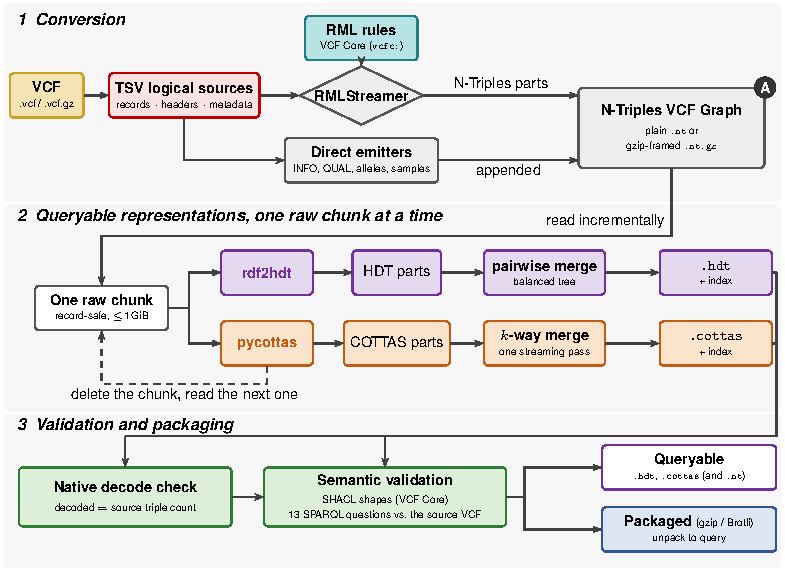
\includegraphics[width=0.92\textwidth]{figs/vcf2rdf-v3.pdf}
\par\medskip
\figcaption{\textbf{Figure 1. What the tool does} (main Figure~2). (1)~A VCF is split into tabular logical sources, mapped by RML rules and direct emitters, and written as one N-Triples VCF graph. (2)~The graph is turned into HDT and COTTAS one raw chunk at a time, then merged. (3)~A native decode check confirms each artifact's triple count against the graph, and semantic validation compares thirteen SPARQL questions with the source VCF and applies SHACL shapes.}
\end{figure}

\section{2. What changed since the 8 October brief}

\begin{itemize}
\item \textbf{A condensed manuscript.} The condensed version is now the manuscript, and the full-length draft is retired. The main text keeps six figures (the VCF Core terms, the pipeline overview beside the section it explains, the validation outcomes, the workflow matches, the converter comparison, and the cost of querying) and the representation-contract table. The workflow's stage costs, the sample ladder, and the detailed retrieval paths move to Supplementary Figures~S3, S5 and~S7.
\item \textbf{Evaluation design beside its results.} Section~3 now combines the evaluation design with the results: each research question's subsection describes how it was tested and then what the tests showed, so no method has to be looked up in a separate section.
\item \textbf{Every reported result comes from a published release.} The base campaign used v3.1.0. Everything a pre-release build first produced was rerun with the published v3.3.1: use-case Arms~1--3, regional retrieval, large-graph retrieval, and the consumer WGS validation run. Every match set and carrier list is identical. Timings moved by a few percent, and no conclusion changed:
  \begin{itemize}
  \item the complete HG005 VCF now takes 646.4\,s of queries after an 881-second index, against 634.6\,s and 868\,s before;
  \item Arm~3's queries now take 216--218\,s, against 205--209\,s before.
  \end{itemize}
  The two releases write identical graphs, so the v3.1.0 graphs that the retrieval experiments query stand for v3.3.1's. Arm~4's rerun finished on 10 October with the same matches, released records, and links as before; only its timings changed, on another host.
\item \textbf{Records compared in every arm.} The rerun compares the records each view releases, as well as the matches. Arms~1, 3 and~4 agree record for record. Arm~2's research views released 110 (DS) and 58 (GRU) symbolic structural-variant records in restricted cancer-predisposition genes, because v3.3.1 cannot link a symbolic allele to a gene. No match changed. RQ2 now reports this, and the Scope section keeps it as a limitation.
\item \textbf{The MyVariant.info result reproduced.} v3.3.1 reproduces the one live-service result (92--93\% of rsIDs confirmed) from the 21 responses recorded on 28 September, without querying the service again. The responses are published with the archive.
\item \textbf{The archive is ready for Zenodo.} The testing repository has been cleaned of unused files and internal notes, and documented. Its results README maps every figure and table to its run records and release.
\end{itemize}

\subsection{Earlier in this revision (8 October)}
\begin{itemize}
\item \textbf{Structure.} Implementation, Evaluation and Results each followed RQ1--RQ3. The \emph{base campaign} (143 runs in 12 experiment families, v3.1.0) is defined where it is first used and detailed in Supplementary Section~S6.1.
\item \textbf{Setup counted for what QLever needs.} The break-even counts conversion to the gzip-framed N-Triples that QLever indexes, not HDT: about 2\,min of setup and 11 questions, instead of 7.4\,min and 44. The N-Triples are 21--25$\times$ the gzipped VCF.
\item \textbf{A fourth workflow arm.} Arm~4 applies layered rules to the complete NB72462M VCF (5,063,417 records), giving four requesters four different, non-empty release views.
\item \textbf{Spanning deletions linked.} v3.3.1 links spanning-deletion (\texttt{*}) records to genes by their REF span; v3.3.0 did not, so gene-based rules could not select them.
\item \textbf{The consumer WGS validation run passes.} Its three earlier mismatches were validator gaps (uncounted phase sets; QUAL compared as written), corrected in v3.3.1. The failure history is in Supplementary Section~S4.2 only.
\item \textbf{A shared-input converter comparison} with JVarkit, TogoVar, SPARQLing Genomics and BioInterchange (Section~5 below), rerunnable with one Docker Compose command.
\item \textbf{A stated SHACL limitation.} Full shape validation does not yet scale to the graph of a complete single-sample VCF (Section~3 below).
\item \textbf{Title and naming.} ``Policy-aware'' replaces ``Governable''. A VCF file is never called a ``genome'': inputs are named by file and record count, and the VCF side is described as \emph{VCF parsing} or \emph{region queries on a tabix-indexed VCF}.
\end{itemize}

\section{3. RQ1: source comparisons and structural validation are complementary}

On valid inputs every check agreed with an answer derived independently from the source VCF: all 1,006 applicable query comparisons of the base campaign's 78 validation runs, the decoded triple count of all 152 HDT and COTTAS artifacts, all thirteen answers on the 657.4M-triple graph of the complete HG005 VCF, and all thirteen in the consumer WGS validation run (58.2M triples). The 25 runs repeated on four SPARQL engines returned identical answers.

On 113 injected faults, the queries detected 96. The default shapes detected none of the remaining 17, which change relationships no query summary inspects (which allele a genotype refers to, a sample's index, phasing, header attribute values); the two deeper profiles detected all of them.

\begin{figure}[!htb]
\centering
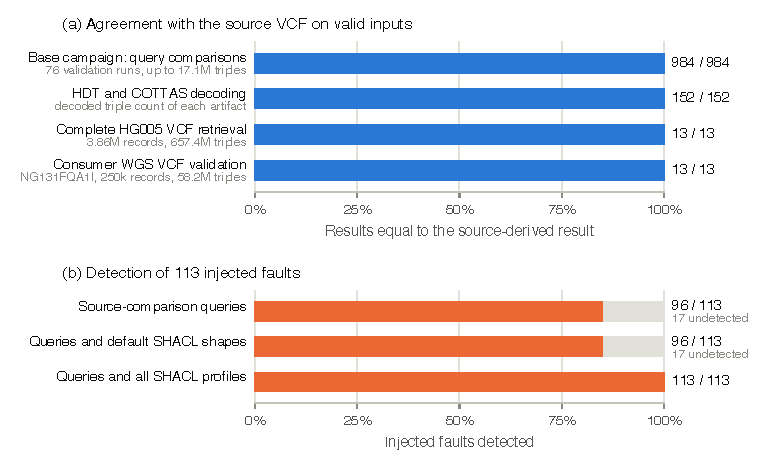
\includegraphics[width=0.9\textwidth]{figs/fig-validation.pdf}
\par\medskip
\figcaption{\textbf{Figure 2. Validation outcomes on valid inputs and on injected faults} (main Figure~3). Each bar spans the expected outcome and is filled to the observed one. (a)~Agreement with source-derived answers. (b)~Detection of 113 injected faults by the queries alone, with the default shapes, and with all shape profiles.}
\end{figure}

\subsection{The new limitation: shape validation at scale}
The SHACL engine holds the graph in memory at about 2.4\,GB per million triples. The default profile's constraints are local to a record, so it now runs in record batches: 91 minutes for the 58.2M-triple graph, or about 17 hours at that rate for the 657.4M-triple graph of the complete HG005 VCF. The deeper profiles compare records with one another and must see the whole graph, so on the 31\,GB benchmark hosts they are capped at 10M triples, and their running time on large graphs is unmeasured. The fault coverage they add is therefore not yet available for complete VCFs; the paper names this as future work.

\subsection{What matters beyond pass counts}
During development the validation found three real defects that a record count could not have shown: a header-only file omitted its declared samples; genotypes referred to allele resources a raw-INFO conversion never emitted; and withheld files left their headers in release views.

\reading{main Sections~3.1 and~4.5; supplement Sections~S4 and~S8.}

\section{4. RQ2: the same answers, with explicit and reusable relationships}

The workflow asks which observed variants in the frozen 81-gene ACMG SF v3.2 set have a ClinVar classification (at least one review star), with which participant and gene, and which matches each requester may receive. Policies are simulated. Counts are participant--variant--gene matches, not people, and the pathogenic or likely pathogenic subset (zero in Arms~1, 3 and~4; eight in Arm~2) is not a set of clinically adjudicated findings.

\begin{figure}[!htb]
\centering
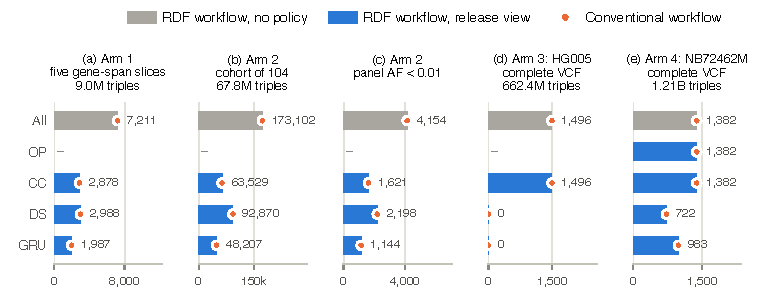
\includegraphics[width=\textwidth]{figs/fig-usecase-matches.pdf}
\par\medskip
\figcaption{\textbf{Figure 3. Identical match sets for every requester in every arm} (main Figure~4). Bars are the RDF workflow and dots the bcftools workflow. Arm~1: the ACMG gene-span regions of five single-sample VCFs; Arm~2: 104 1000~Genomes participants, with a separate panel-frequency graph in (c); Arm~3: the complete HG005 VCF; Arm~4: the complete NB72462M VCF. All: no policy; OP: the participant's own physician; CC: clinical care; DS: cardiovascular research; GRU: general research use.}
\end{figure}

\begin{itemize}
\item \textbf{Agreement.} Every requester-specific match set equals the conventional workflow's, and every materialized release view passed the policy and source checks. Arm~3's complete HG005 VCF reproduced its Arm~1 gene-span result (1,496 matches). The records each view released also agree in Arms~1, 3 and~4.
\item \textbf{The structural-variant gap (Arm~2).} v3.3.1 links no symbolic allele or breakend to a gene, so the cancer-gene restriction cannot select such records. Arm~2's research views therefore released 110 (DS) and 58 (GRU) symbolic structural variants in restricted genes that the bcftools workflow withheld. No match changed, because the case definition joins explicit alleles only. The paper states the gap (main Sections~3.2 and~4.7); a fix that links these records by their REF span is not yet in a release.
\item \textbf{Fine-grained release (Arm~4).} OP received every record; CC all but six APOE records; GRU all but 2,520 records under the cancer-gene, APOE and single-variant rules; DS only the 6,397 records in its cardiovascular panel.
\item \textbf{Shared information stored once.} A separate 68,635-site graph of 6.5M triples replaces about 857M triples of panel INFO repeated in each 1000~Genomes participant file (93\% of their RDF). The saving comes from factoring the input, not from RDF compression.
\item \textbf{The live linking tier.} MyVariant.info confirmed 92--93\% of the PGP files' rsIDs. v3.3.1 reproduces this from the 21 responses recorded on 28 September, which are published for anyone to replay.
\item \textbf{Rule changes.} Restricting HFE C282Y to clinical care changed only policy data in the RDF workflow, and also caught an HG002 record on contig \texttt{6} rather than \texttt{chr6}; the conventional workflow needed a code and data edit. This is a change-location demonstration, not a usability claim.
\end{itemize}

\begin{figure}[!htb]
\centering
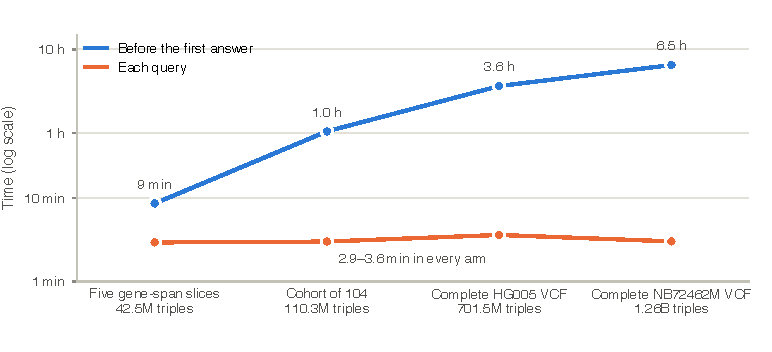
\includegraphics[width=0.9\textwidth]{figs/fig-usecase-costs.pdf}
\par\medskip
\figcaption{\textbf{Figure 4. Setup grows with the data; querying does not} (Supplementary Figure~S3). Time before the clinical-care requester's first answer (convert and link, then write, check, and index its view) against the median query time. Sizes are the triples indexed for each arm's unrestricted query, including the 33.1M-triple ClinVar subset and all links.}
\end{figure}

For Arm~3, converting the complete HG005 VCF and ClinVar took 55\,min, linking 8\,min, and the clinical view a further 2.6\,h (70\,min of it validation), peaking at 11.2\,GB of host memory and 31\,GB of disk. Queries then took 171--233\,s in every arm, dominated by the fixed ClinVar join.

\subsection{Important boundaries}
SPDI joins assume the tested reference, normalization, and eligible allele classes; contig-alias handling is demonstrated, canonical identity across every equivalent representation is not. Every participant is a single-sample VCF, so masking samples within a multi-sample VCF is untested. Consents are simulated, and deployment security and real consent validity remain separate questions.

\reading{main Sections~2.3, 3.2 and~4.4; supplement Section~S5.}

\section{5. RQ3: costs depend on the workload, not on one headline number}

Neither route is uniformly cheaper. VCF parsing wins one-pass analyses and small regions on a tabix-indexed VCF; RDF querying wins large regions, whole-file questions asked one at a time, and, once its setup of about two minutes is paid, repeated questions. The graph route costs storage as well as time: the N-Triples QLever indexes are 21--25$\times$ the gzipped VCF. The sample representation decides how much graph there is, and triple counts alone overstate that difference.

\begin{figure}[!htb]
\centering
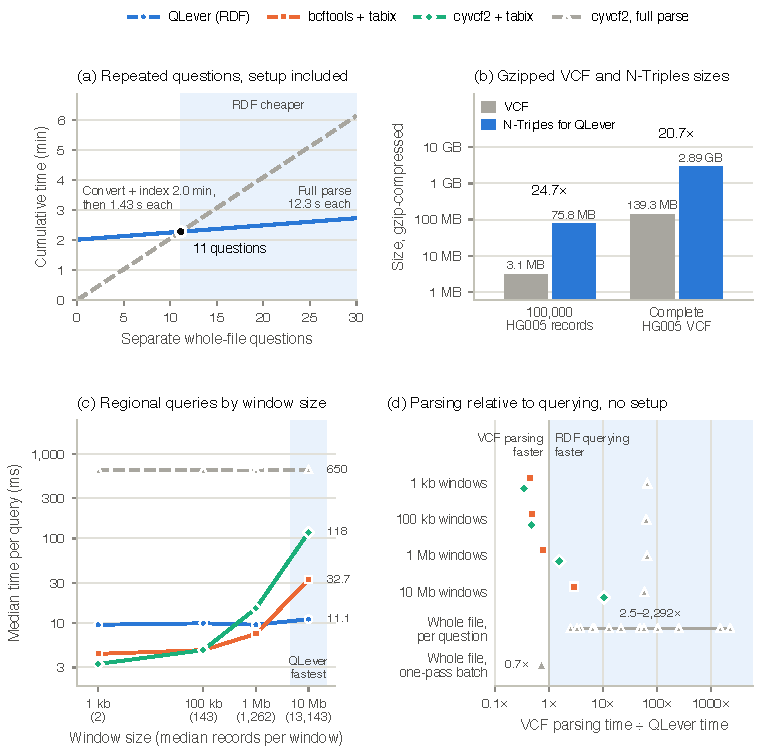
\includegraphics[width=0.95\textwidth]{figs/fig-regional.pdf}
\par\medskip
\figcaption{\textbf{Figure 5. Where VCF parsing is and is not faster than RDF querying} (main Figure~6). All panels use 100,000 HG005 records. (a)~Repeated whole-file questions with setup included: a full cyvcf2 parse per question against 2.0\,min, measured in a rerun, to convert the records to gzip-framed N-Triples and index them in QLever, breaking even at 11 questions. (b)~Gzip-compressed sizes of the VCF and of the N-Triples QLever indexes, also for the complete HG005 VCF. (c)~Median time per regional query by window size (median records per window in parentheses). (d)~Every comparison as VCF parsing time divided by QLever time, setup excluded; points in the shaded region are those where VCF parsing was slower.}
\end{figure}

\begin{center}\small
\begin{tabularx}{\textwidth}{@{}>{\raggedright\arraybackslash}p{0.27\textwidth}X@{}}
\toprule
\textbf{Workload or choice} & \textbf{Finding to retain}\\
\midrule
Single whole-file questions & QLever took 0.005--4.62\,s per question against 11.5--12.3\,s for a full cyvcf2 parse, on 100,000 HG005 records (17.1M triples).\\
All thirteen in one pass & One parsing pass took 12.4\,s; QLever's queries took 17.1\,s, plus a 22.8\,s index.\\
Repeated questions & About 11 questions to break even, measured in a three-replicate rerun: 95.7\,s to convert to gzip-framed N-Triples (HDT is not needed by QLever) and 25.0\,s to index. One scenario, not a tool constant; with the base campaign's HDT it was 44.\\
Storage & The gzip-framed N-Triples QLever indexes are 24.7$\times$ the gzipped VCF for 100,000 records and 20.7$\times$ for the complete HG005 VCF (2.89\,GB against 139.3\,MB).\\
Regional lookups & Tabix-indexed region queries were faster up to 100\,kb (3.2--4.6\,ms against 10.6--10.8\,ms); at 10\,Mb QLever's 10.3\,ms beat bcftools (31.5\,ms) and cyvcf2 (118.2\,ms).\\
Sample representation & At 2,504 samples, expanded output has 432$\times$ the triples of condensed but only 69$\times$ the HDT bytes; condensed values need decoding to address one call.\\
Optional artifacts & Converting the complete HG005 VCF with v3.1.0 took 16.07\,h, about 14.5\,h of it building HDT and COTTAS. These are optional; gzip-framed N-Triples alone occupied 2.89\,GB.\\
Large graphs & On the complete HG005 VCF (657.4M triples), QLever answered all thirteen questions in 646.4\,s after an 881-second index; the native HDT and COTTAS paths did not complete on 171M triples.\\
\bottomrule
\end{tabularx}
\end{center}

\begin{figure}[!htb]
\centering
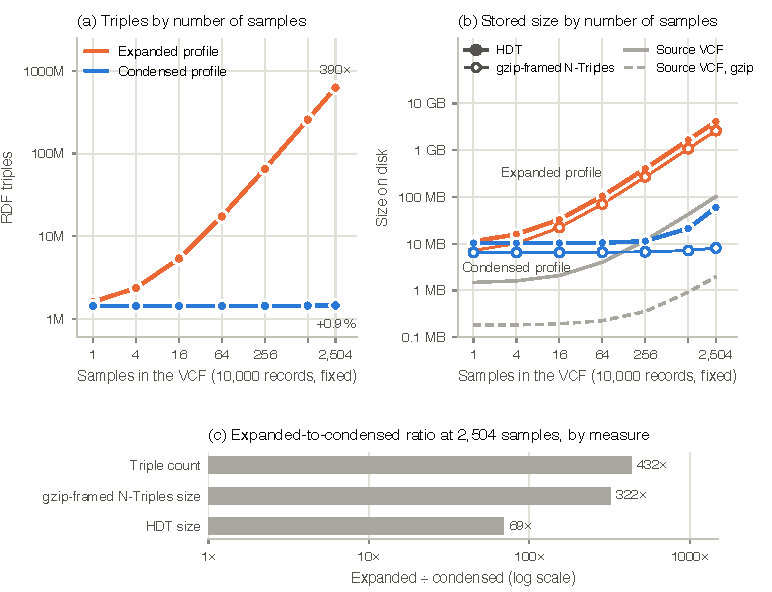
\includegraphics[width=0.85\textwidth]{figs/fig-samples.pdf}
\par\medskip
\figcaption{\textbf{Figure 6. Sample representation trades addressability for size} (Supplementary Figure~S5). 10,000 records of the 1000~Genomes chromosome-20 VCF with one to 2,504 of its samples. (a)~Expanded triples grow 390$\times$ across the ladder, condensed ones 0.9\%. (b)~Stored size of HDT and gzip-framed N-Triples for each profile, beside the source VCF uncompressed and gzip-compressed. (c)~At 2,504 samples, expanded output has 432$\times$ the triples of condensed but 69$\times$ the HDT bytes.}
\end{figure}

Keep the configurations apart: the 16.07-hour v3.1.0 conversion and the 55-minute use-case conversion differ in configuration and are not alternative measurements of the same task.

\subsection{Other converters on the same inputs}
The converter comparison sits in RQ3 because it weighs what a representation holds against what it costs. On the same two inputs, the other converters' graphs held 14--203 triples per record against VCF-RDFizer's 171 (HG005) and 536 (16 samples), and converted each slice in 0.1--6.3\,s against VCF-RDFizer's 31--92\,s, which includes starting a container per stage. None of them answered all eight content questions as the oracle did on both inputs, and every difference traces to what its graph holds, not to how it was queried. It shows what each graph can answer, not which converter suits a given purpose: TogoVar, for one, omits samples by design.

\begin{figure}[!htb]
\centering
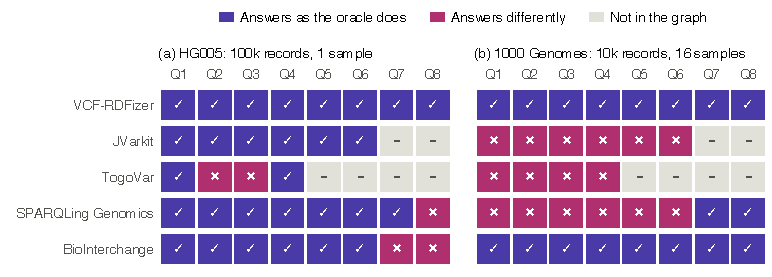
\includegraphics[width=\textwidth]{figs/fig-converters.pdf}
\vspace{2pt}
\figcaption{\textbf{Figure 7. Only VCF-RDFizer's graphs answered every content question as the oracle did on both shared inputs} (main Figure~5). Each cell is one of the content questions Q1--Q8, ported to the converter's vocabulary and answered from its graph: \checkmark\ as the oracle, $\times$ differently, -- not in the graph. Q1--Q4 summarize records, Q5--Q6 genotypes, and Q7--Q8 the header. (a)~100,000 HG005 records, one sample. (b)~10,000 records and 16 samples of the 1000~Genomes chromosome-20 call set. JVarkit merges records sharing CHROM, POS, and REF; TogoVar drops symbolic and \texttt{*} alleles and writes no samples or header; SPARQLing Genomics writes only carriers' calls (1,401 of 10,000 cohort records); BioInterchange's HG005 header document is invalid JSON.}
\end{figure}

\reading{main Sections~3.3 and~4.6; supplement Sections~S2, S9 and~S10.}

\section{6. Coauthor decisions and submission work}

\subsection{Essential: close before submission}
\begin{itemize}
\item \textbf{Persistent archive.} The testing repository is cleaned and documented, and every reported run is archived in it. Deposit it in Zenodo and reserve its DOI for the Availability statement.
\item \textbf{Declarations.} Complete the funding statements for B.B., R.T., and G.E., and confirm the separation from the companion VCF Core vocabulary paper.
\end{itemize}

\subsection{Presentation choices to confirm}
\begin{itemize}
\item The condensed main text keeps six figures, with the pipeline overview in Section~2.2; the stage costs, sample ladder, and detailed retrieval paths are supplementary (S3, S5, S7).
\item The consumer WGS validation run is reported in the main text by its corrected-validator result alone, with the earlier failures and their diagnosis only in the supplement.
\item Arm~2's structural-variant gap is reported as a limitation of the published v3.3.1, rather than removed by an unreleased fix.
\item Arm~4 and the v3.3.1 linker fix are minimal in the main text and detailed in Supplementary Section~S5.
\item The SHACL scaling limit is framed as future work rather than as a weakness of the validation design.
\item The break-even is computed for the N-Triples QLever indexes, with HDT and COTTAS treated as optional artifacts; the regional medians behind main Figure~6 are in Supplementary Table~S18.
\end{itemize}

\subsection{Claim-dependent additions, not an automatic new benchmark campaign}
\textbf{External relevance.} Would a focused clinical or data-access review of the application question strengthen the contribution? The shared-input converter comparison is now in the paper (Figure~7 here), but it covers four converters, two inputs, and Q1--Q8, so it shows what each graph can answer rather than which converter suits a purpose. The bcftools comparison is a task comparison, not a converter benchmark, and there is no user study.

\end{document}
